%%%%%%%%%%%%%%%%%%%%%%%%%%%%%%%%%%%%%%%%%%%%%%%%%%%%%%%%%%%%%%%%%%%%%%%%
% Plantilla TFG/TFM
% Escuela Politécnica Superior de la Universidad de Alicante
% Realizado por: Jose Manuel Requena Plens
% Contacto: info@jmrplens.com / Telegram:@jmrplens
%%%%%%%%%%%%%%%%%%%%%%%%%%%%%%%%%%%%%%%%%%%%%%%%%%%%%%%%%%%%%%%%%%%%%%%%

\chapter{El motor gráfico}

Antes siquiera de poder empezar a desarrollar la primera demo, es necesario crear un entorno que sea capaz de automatizar las tareas más básicas que no son competencia directa de la demo, como por ejemplo gestión de la ventana y de las entradas de teclado. Este código será común y necesario a todas las demos, pues independientemente de sus características concretas, todas ellas necesitarán una ventana y un espacio en el que poder volcar datos.\\

Es por ello que antes de empezar con la primera demo, se hizo necesario el desarrollo de un pequeño \emph{framework} que permitiese gestionar de la forma más rápida y sencilla posible aquellas tareas que no debían ser responsabilidad directa de la demo. 

\section{Investigación inicial}

Una de las principales influencias en el desarrollo de la versión inicial del motor gráfico fue OneLoneCoder\footnote{\url{https://www.youtube.com/channel/UC-yuWVUplUJZvieEligKBkA}}. Este programador británico tiene una colección de tutoriales con alto valor educativo y en muchos de ellos explica incluso técnicas de programación de la vieja escuela. Fue a raíz de visualizar estos vídeos donde vi expuestos muchos de los problemas a los que me tendría que enfrentar en el futuro.\\

El ejemplo más claro: en sus primeros vídeos, este programador siempre repite el mismo código para poner en marcha una consola usable, hasta que decide crear un modelo básico que le permita reutilizar este código.\\

Este canal ha tenido un gran valor formativo para mí, ya que me permitió identificar una serie de problemas que de otro modo sólo hubieran aparecido en un momento más avanzado del desarrollo, y que sin embargo, hubieran resultado costosos de solventar.\\

Inicialmente, estos fueron los objetivos que pretendía cubrir el motor gráfico:
\begin{itemize}
	\item \textbf{Reutilización de código}: tareas como abrir y cerrar la ventana o gestionar el dibujado son necesarias en absolutamente todas las demos, por lo que todo código relacionado con la ventana y/o el dibujado debería poder ser reutilizado sin tener que duplicarse.
	\item \textbf{Encapsulación de toda lógica no relacionada con la demo}: uno de los principales objetivos que se persiguen con la creación de un motor gráfico es la claridad. La implementación de una demo \textbf{sólo debe contener lógica que está directamente relacionada con sus detalles de implementación}, es decir, con los algoritmos o técnicas de los que la demo hace uso. De este modo, el código de una demo sólo refleja la lógica de la misma, sin exponer la lógica necesaria para la de gestión de ventana, que no es responsabilidad de la misma. Esto permite un código más claro y conciso, más fácil de implementar, usar, refinar y entender.
		\begin{itemize}
			\item \textbf{Encapsulación de la ventana}: una demo no debe ser consciente de qué es necesario para crear o borrar una ventana, todo lo que debe hacer es ser poder decir "quiero crear una ventana" o "quiero cerrar la ventana" pero no debe ocuparse de los detalles de implementación.
			\item \textbf{Encapsulación del dibujado}: una demo no debe tener responsabilidad de gestionar el dibujado en ventana. Todo lo que una demo necesita saber es en qué lugar de memoria debe escribir para que esos datos sean dibujados en pantalla, pero no debe encargarse de la gestión del dibujado.
		\end{itemize}
	\item \textbf{Abstracción de la plataforma}: el código de una demo no debe contener detalles de implementación relativos a la plataforma en que se ejecuta. Desde el punto de vista de la demo, todo lo que importa es el algoritmo, y este debe ser el mismo independientemente del sistema operativo y del \emph{hardware} sobre el que se ejecuta.
\end{itemize}

Durante el desarrollo, no obstante, nuevas necesidades se irían añadiendo, ya fuera por nuevas decisiones de diseño, refinamiento de código o por nuevas necesidades de las demos:
\begin{itemize}
	\item \textbf{Abstracción de las librerías y tecnologías utilizadas}: tras varias iteraciones sobre el desarrollo inicial, fue necesario un refinamiento. El motor gráfico contenía demasiada lógica, y era lógica acoplada a la gestión de la ventana o del dibujado. Esto levantó una pregunta: ¿y si en algún momento necesito cambiar las librerías que utilizo o incluso prescindir de las mismas? Esta era una posibilidad bastante probable, dado que a lo largo del desarrollo de un proyecto y conforme surgen nuevas necesidades, puede que las tecnologías elegidas inicialmente no satisfagan las condiciones actuales. Por tanto, el motor gráfico no debía estar acoplado a las tecnologías que usaba, si no que debía mediar con ellas mediante el uso de interfaces.
	\item \textbf{Abstracción de los eventos de teclado}: conforme el desarrollo avanzó, se hizo aparente que en muchas ocasiones era útil permitir al usuario modificar parámetros de la demo en tiempo real, en cierto modo permitir "jugar" con la demo. Era necesario por tanto permitir el manejo de eventos de teclado, aunque su uso debía estar abstraído de su implementación, de forma que desde el punto de vista de la demo, todo lo que se pudiera hacer es "quiero saber el estado de esta tecla".
	\item \textbf{Abstracción del dibujado de texto en pantalla}: una vez más, al continuar con el desarrollo, se hizo aparente la necesidad de poder dibujar texto en pantalla. El motor gráfico debía ser por tanto capaz de abstraer o enmascarar las rutinas de dibujado del texto, de modo que desde la perspectiva de la demo todo lo que importase fuera dibujar un texto con un color, posición y tamaño determinados, independientemente de la implementación.
	\item \textbf{Uso de mecanismos de dibujado seguros para formas básicas}: aunque inicialmente parecía que cualquier tipo de dibujado debía ser responsabilidad de la demo, pronto se hizo aparente que ciertas rutinas se repetían de forma constante. Además, mientras que en un inicio el dibujado de un punto o una línea era responsabilidad de la demo, pronto se vio que desde el punto de vista de la demo, estas responsabilidades no tienen interés, ya que la capacidad de poder dibujar una línea es importante, pero no cómo se dibuja. 
		\begin{itemize}
			\item \textbf{Dibujado de puntos}: desde la perspectiva de una demo, tan sólo importan la posición, color y tamaño de un punto que se quiera dibujar en pantalla. La gestión de si ese punto está dentro o fuera de los límites de pantalla o la gestión del tamaño del punto no debería ser competencia de la demo, si no del motor.
			\item \textbf{Dibujado de líneas}: una demo debe ser capaz de solicitar el dibujado de una línea dados dos puntos, un color y un tamaño, pero no debe responsabilizarse de la gestión de los límites en pantalla ni del algoritmo de dibujado para una línea.
			\item \textbf{Dibujado de rectángulos}: una demo debe ser capaz de dibujar rectángulos en pantalla, especialmente útiles para el borrado de la pantalla o de regiones de la misma, pero no debe conocer sus detalles de implementación.
		\end{itemize}
\end{itemize}

Con todos estos puntos en mente, y de forma progresiva, se fue desarrollando, revisando y refinando la creación de un motor gráfico que sirviera como marco de trabajo efectivo para el desarrollo de una demo.

\section{Características}

%@startuml
%
%abstract ClassicDemoTemplate {
%  .. Public methods ..
%  +Construct(name, width, height, fullscreen)
%  +Run()
%  +Close()
%  .. Methods usable by children ..
%  #GetWindowManager()
%  #RenderDot(position, colour, size)
%  #RenderLine(position, colour, size)
%  #ClearScreen(square, colour)
%  #IsPixelOutOfBounds(position)
%  .. Pure virtual methods overriden by children ..
%  -Init()
%  -Update(deltaTime)
%  -Destroy()
%}
%
%interface IWindowManager {
%  +CreateWindow(name, width, height, fullscreen)
%  +UpdateWindow()
%  +DestroyWindow()
%}
%
%interface IRenderManager {
%  +InitialiseRender(width, height)
%  +DrawToScreen()
%  +DisposeRender()
%}
%
%class OpenGLRenderManager {
%}
%
%class GLFWWindowManager {
%}
%
%OpenGLRenderManager -|> IRenderManager
%GLFWWindowManager --|> IWindowManager
%
%IRenderManager -* GLFWWindowManager
%ClassicDemoTemplate *- IWindowManager
%
%hide empty members
%
%@enduml

\begin{figure}[h]
	\centering
	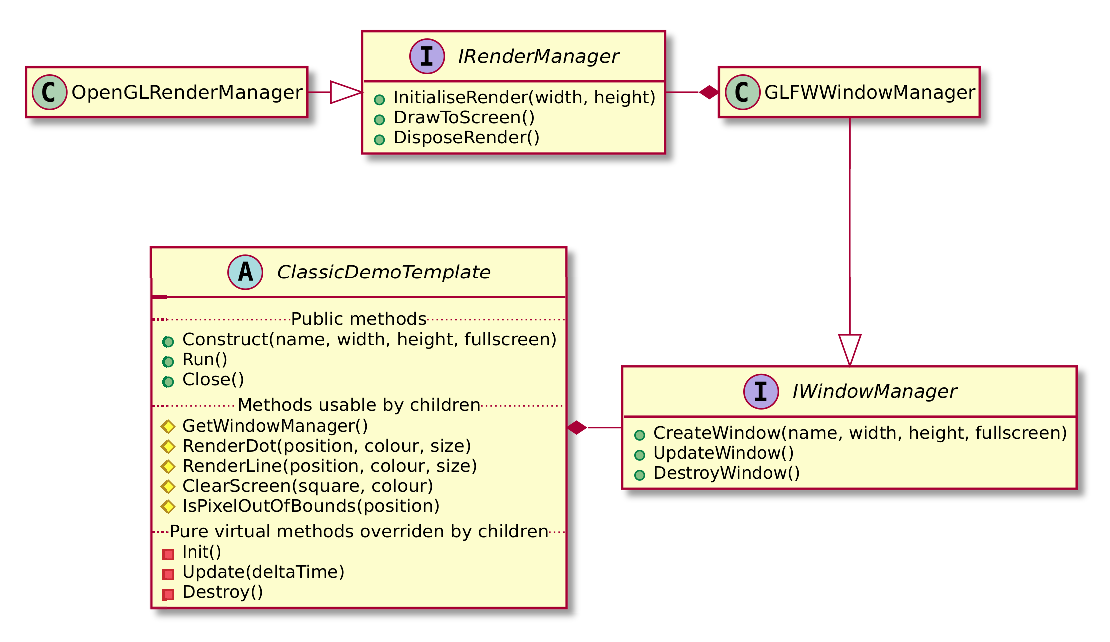
\includegraphics[width=15cm]{archivos/classicdemotemplateuml}
	\caption{Diagrama simplificado de la estructura del motor gráfico}
	\label{fig:classicdemotemplateuml}
\end{figure}

La figura [\ref{fig:classicdemotemplateuml}] presenta la estructura simplificada del motor gráfico.\\

Como se puede observar, el motor (\emph{ClassicDemoTemplate)} delega las tareas de gestión de la ventana en una interfaz cuyos métodos más relevantes permiten crear, actualizar y destruir la ventana. De este modo, el motor gráfico está completamente desacoplado de las tareas concretas de gestión de la ventana.\\

La implementación concreta de la interfaz (\emph{GLFWWindowManager}) utiliza, como su nombre indica, la librería GLFW para gestionar la ventana. Esta es una librería de código abierto y multiplataforma que hace más sencilla la gestión. No obstante, la implementación concreta está completamente desacoplada del sistema, por lo que si fuera necesario migrar a una tecnología distinta (como SDL, SFML o accediendo directamente a la API gráfica de Windows (WinAPI) o Linux (X11)), se podría hacer siempre y cuando esta nueva clase implementase la interfaz definida.\\

A su vez, \emph{GLFWWindowManager} hace uso de la interfaz \emph{IRenderManager}, que implementa \emph{OpenGLRenderManager}. Esto permite, una vez más, cambiar la tecnología de dibujado sin tener que cambiar necesariamente el sistema de ventanas. De este modo también se separa de forma efectiva todo el código relativo a la gestión de la ventana con respecto al código relativo al dibujado, lo que facilita la claridad y mantenimiento del código.\\

En nuestro caso, el dibujado se hace mediante OpenGL, una especificación para gráficos 3D multiplataforma. No obstante, OpenGL es utilizado como un mero mediador, cuyo único uso es el dibujado de una textura en pantalla. Es esta textura que se \emph{renderiza} de forma cíclica a la que el usuario tiene acceso y puede modificar, dibujando así en pantalla.\\

De este modo, la clase principal de nuestro motor \emph{(ClassicDemoTemplate)} no tiene responsabilidad directa sobre la gestión de la ventana y el dibujado, de modo que aunque las librerías o tecnologías utilizadas cambiasen, toda la lógica contenida en el motor seguiría siendo usable.\\

Como se puede observar en el diagrama, esta clase principal es una clase abstracta, lo que implica que debe ser implementada por una clase concreta para poder instanciarse. Toda demo que use este motor gráfico debe heredar de \emph{ClassicDemoTemplate}. Esto permite definir una estructura que todas nuestras demos deberán satisfacer para hacer un uso efectivo de nuestro motor.\\

En primer lugar, se exponen únicamente tres métodos, \emph{Construct}, \emph{Run} y \emph{Close}. Esto implica que cualquier demo ha de ser completamente usable mediante estos tres métodos.\\

A continuación, \emph{ClassicDemoTemplate} expone una serie de métodos que pueden ser utilizados únicamente por las demos, que heredan de esta clase. Estos métodos aportan funcionalidad común que resultan útiles en la mayor parte de las demos, como dibujar puntos y líneas o comprobar si un píxel determinado está dentro de los límites de la ventana.\\

Por último, hay tres métodos virtuales y privados que toda demo debe implementar: \emph{Init}, \emph{Update} y \emph{Destroy}. La llamada a estos método es gestionada por \emph{ClassicDemoTemplate}, por lo que el usuario tan sólo debe preocuparse de implementarlos. Los métodos \emph{Init} y \emph{Destroy} permiten inicializar y destruir las variables los datos propios de la demo. El método \emph{Update} es llamado en el bucle de ejecución del programa y recibe el tiempo sucedido desde el último fotograma. Este método contendrá toda la lógica necesaria para actualizar los datos que maneja nuestro programa a lo largo del tiempo. 

\subsection{La textura de dibujado y el píxel}

Para dibujar en pantalla en este proyecto, lo único que nos interesa es tener una zona de memoria en la que sepamos que podemos volcar datos. Es decir, no se usarán librerías externas para manipular los gráficos que se muestran en pantalla, si no que todas las transformaciones y el pintado en pantalla corre a nuestra cuenta.\\

Para ello, no obstante, el motor debe tener la capacidad de proveernos con un espacio de memoria en el que podamos pintar. Esto es responsabilidad de la implementación del \emph{IRenderManager.}\\

En nuestro caso, la clase \emph{OpenGLRenderManager} crea una textura basada en la altura, anchura y número de canales que queremos usar para la demo.\\

La altura y anchura se define en píxeles, y el número de canales se corresponde con la cantidad de canales de color que queremos. Por ejemplo, si quisiéramos un ventana monocromática, bastaría con definir un solo canal. Para crear una ventana que pueda representar (casi) cualquier color, necesitamos definir tres canales: rojo, verde y azul. Estos son los tres colores primarios de la luz. A través de combinaciones de los mismos podemos crear cualquier color. También podríamos definir incluso cuatro canales, tres para el color y un canal \emph{alfa} para la transparencia. Por defecto, se crea una textura asumiendo tres canales, cada uno de 8 bits, por lo que disponemos de 256 intensidades de color por canal y un total combinado de 16777216 colores posibles. La memoria reservada es pasada cada fotograma a OpenGL, como una textura. Es entonces estas librería la que se encarga de volcar estos datos en pantalla.\\

Sin embargo, desde el punto de vista del usuario, trabajar con la memoria directamente se hace, cuanto menos, incómodo. Para poder modificar cualquier píxel en pantalla es necesario tener en cuenta el número de canales, la posición y orden de cada color para un píxel determinado... y de pronto operar con píxeles, que debería ser algo sencillo, se convierte en una tarea compleja. Para poder sumar dos píxeles de pronto hay que sumar manualmente cada canal por separado, ¿pero qué pasa si la suma de dos canales supera el valor máximo que puede tener un color por canal, 255? La suma binaria de 128 más 128 resultaría en 0, con lo que si intentamos sumar dos rojos de intensidad media, obtendríamos como resultado el color negro (0), en lugar de un rojo intenso (255). Manejar esta textura se convierte de pronto en una tarea poco intuitiva, que nos llevará a cometer errores con mayor facilidad. Es por ello que se introduce el concepto del píxel a nivel del código.\\

%@startuml
%
%class Pixel
%{
%  + R
%  + G
%  + B
%  +Pixel()
%  +Pixel(value)
%  +Pixel(r, g, b)
%  +Pixel operator+(Pixel)
%  +Pixel operator-(Pixel)
%  +Pixel operator*(float)
%}
%
%hide empty members
%
%@enduml

\begin{figure}[h]
	\centering
	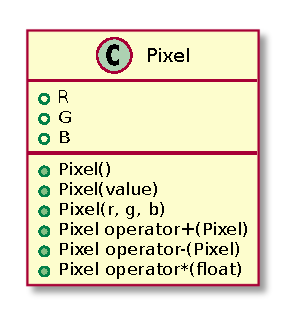
\includegraphics[width=6cm]{archivos/pixeluml}
	\caption{Estructura de un píxel en el motor gráfico}
	\label{fig:pixeluml}
\end{figure}

Un píxel [\ref{fig:pixeluml}] es una clase que contiene únicamente tres variables cuyo acceso es público. Estas variables son R(ed), G(reen) y B(lue), haciendo referencia al nombre del color (en inglés) asociado a cada canal. De este modo, la representación de un píxel coindide en memoria con la textura que hemos definido. De este modo, si bien a OpenGL le pasamos un conjunto de bytes, desde nuestro sistema los podemos organizar en píxeles.\\

Se proveen tres posibles constructores para un píxel. El constructor por defecto inicializa todos los valores a 0 (es equivalente a crear un píxel negro). También podemos proveer un solo valor al constructor, en cuyo caso se asignará este valor a cada canal (resultando en un color gris de mayor o menor intensidad) y por último podemos inicializar un píxel proveyendo un valor específico a cada canal. Es importante notar que por razones de eficiencia y simplicidad, no se hace ningún tipo de comprobación en la construcción, por lo que el intento de asignación de cualquier valor fuera de rango será equivalente al módulo de 256 de dicho valor. Por ejemplo, si intentamos asignar el valor 512 a un canal, será equivalente a asignarle un valor de 0.\\

Tras los tres métodos de construcción, se proveen tres operaciones matemáticas que se pueden realizar con píxeles, suma y resta de píxeles y multiplicación de un píxel por un escalar. La división de un píxel por un escalar no se provee ya que no resulta necesaria, en caso de que se quiera dividir el valor de un píxel, se multiplica por el inverso, consiguiendo el mismo resultado.\\

Por razones de consistencia, la suma y resta de píxeles tienen comprobaciones para evitar el desbordamiento. No sería deseable en nuestro sistema que la suma de dos píxeles cualesquiera, por ejemplo (128, 129, 130) y (200, 201, 202), resultara en un color oscuro. La suma de estos dos píxeles resultaría en (255, 255, 255), es decir, en blanco. Del mismo modo, la resta de dos pixeles siempre debería producir un color más oscuro, pero nunca más claro, por lo que cualquier resta de píxeles que pudiera producir desbordamiento (123 - 124 = -1, que equivale a 255, siendo este valor máxima intensidad) se resuelve en 0 (mínima intensidad o negro).\\

La multiplicación de un píxel por un escalar no se comprueba, ya que dado su uso en el sistema, no resulta práctico. El usuario ha de ser consciente, sin embargo, que sólo las operaciones en que el valor del escalar está entre 0 y 1 son seguras, ya que la multiplicación de un píxel por cualquier valor inferior a 0 o superior a 1 puede producir, potencialmente, desbordamiento (64 * 2 = 128, no desborda, comportamiento esperado; 128 * 2 = 256, resulta en 0, comportamiento inesperado).\\

El motivo por el que la suma y la resta son operaciones comprobadas mientras que la construcción y la multiplicación no lo son está justificado. Los valores de construcción y multiplicación en nuestro sistema están siempre controlados, y en la mayor parte de los casos predefinidos, por lo que se asegura de antemano que no se va a producir un desbordamiento, y por tanto poner comprobaciones para estas operaciones tan sólo supondría en la pérdida de eficiencia (ahora bien, es necesario hacer un uso consciente de las mismas). La suma y la resta necesitan comprobaciones ya que la mayor parte de sumas y restas que se producen son sobre valores generados dinámicamente, sobre los que no tenemos control directo, por lo que no podemos asegurar que no se va a producir desbordamiento, y debemos, por tanto, prevenirlo.\\

Del mismo modo, se provee acceso directo al valor de cada píxel, no solo para su lectura, si no también para su escritura. Esto se hace por conveniencia, pues en ocasiones puede que solo queramos modificar un canal concreto. Debe tenerse en cuenta, no obstante, que estas operaciones pueden provocar desbordamiento. La razón de esta decisión es nuevamente el hecho de que cuando se accede de forma directa al valor de un canal, se hace de forma controlada, por lo que se programa en torno a la posibilidad de desbordamiento.\\

Este sistema busca ser eficiente, por lo que sólo se realizan comprobaciones cuando se consideran estrictamente necesarias. Esto fuerza, no obstante, a hacer un uso consciente del sistema.

\subsection{Detectar input}

Por básica que pueda parecer la detección de entradas de teclado, esta característica no fue implementada hasta un estado relativamente avanzado del desarrollo del proyecto. Aunque esto pueda resultar difícil de entender desde el punto de vista del usuario, desde el punto de vista del desarrollador, las entradas de teclado sirven principalmente para "jugar" con la demo y para ajustar valores, es decir, que resultan útiles en el proceso de refinamiento de la demo, pero son irrelevantes en el proceso de creación de la misma. Es por ello que disponer de \emph{input} para las demos no es algo que se priorizara, ya que estaba mucho más interesado en el desarrollo de los algoritmos y métodos necesarios para cada demo que no en poder "jugar" con los resultados.\\

No obstante, llegó un punto en el desarrollo en el que las demos, además de ser funcionales, debían ser manipulables, modificables de forma dinámica, y fue en este momento cuándo se planteó la pregunta de cómo gestionar las entradas de teclado.\\

Las entradas de teclado se gestionan desde la ventana, por lo que tenía claro que su gestión debería ser parte de la responsabilidad de \emph{GLFWWindowManager}. Era importante, sin embargo, saber en qué eventos de teclado estaba interesado.\\

Estos eran los eventos que me interesaban: saber el momento en que la tecla se pulsa por primera vez, saber el momento en el que la tecla se suelta y saber si la tecla se está manteniendo pulsada o no. Sin embargo, GLFW sólo daba acceso directo a saber si la tecla estaba pulsada o no, por lo que la lógica para el resto de eventos debía ser implementada por mi parte.\\

GLFW permitía otra opción, además, en lugar de preguntar por el estado de una tecla concreta, es posible pasarle un método delegado que sea llamado cada vez que se produce un evento, de forma que este método sobre el que nosotros tenemos control pueda gestionar los eventos en los que estamos interesados. Por razones de simplicidad y mantenibilidad, decidí optar sin embargo por la opción de preguntar por el estado de las teclas.\\

Esta opción sin embargo planteaba un problema de eficiencia: la única forma de saber si una tecla cualquiera está pulsada o no es almacenando y actualizando el estado de todas las teclas. Esto implicaría tener que estar actualizando el estado de más de 100 teclas cuando tan sólo tenemos interés en unas pocas. Y precisamente lo que decidí fue añadir un método que permitiera registrar interés en una tecla. Esto hace que la gestión de \emph{input} en una demo sea ligeramente más compleja (para poder preguntar por el estado de una tecla, esta debe haberse registrado previamente). Sin embargo, a cambio de esta ligera complejidad añadida, hay una gran ganancia en rendimiento, ya que en lugar de actualizar el estado de \emph{todas} las teclas del teclado por fotograma, sólo actualizaremos el estado de aquellas que nos interesan, y en caso de no tener interés en ninguna, simplemente no se tendrán en cuenta las entradas de teclado, no impactando en ningún modo al rendimiento del programa.\\

%@startuml
%
%interface IWindowManager {
%  +RegisterKeyInput(key)
%  +IsKeyPressed(key)
%  +IsKeyHeld(key)
%  +IsKeyReleased(key)
%  +IsKeyUp(key)
%}
%
%class KeyState << (S,#FF7700) Struct >>
%{
%  +IsPressed
%  +IsHeld
%  +IsReleased
%  +IsUp
%}
%
%hide empty members
%
%@enduml

\begin{figure}[h]
	\centering
	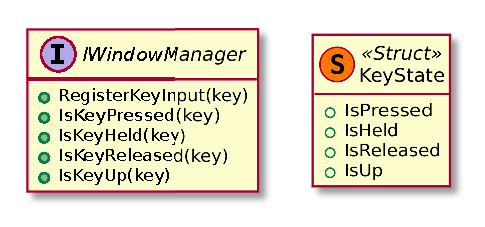
\includegraphics[width=10cm]{archivos/inputuml}
	\caption{Funciones y estructuras del sistema de input}
	\label{fig:input}
\end{figure}

\subsection{Dibujar texto}

Al igual que con el input, la necesidad de dibujar texto no se hizo aparente hasta un estado más avanzado de desarrollo del proyecto. Una vez en la tesitura en la que poder dibujar texto en pantalla era necesario, fue necesario dedicar un tiempo de análisis.\\

Inicialmente pensé en usar una librería y estuve investigando cuál podía satisfacer mejor mis objetivos. glfreetype\footnote{\url{https://github.com/benhj/glfreetype}} parecía bastante adecuada, tratándose de una librería pequeña, concisa y aparentemente sencilla de utilizar.\\

A mitad camino del proceso de integración de esta librería, no obstante, me empecé a plantear hasta qué punto tenía sentido utilizar una librería externa para el dibujado de texto en pantalla. Al fin y al cabo, uno de mis objetivos con este trabajo era que todo aquello que estuviera dibujado en pantalla hubiera sido desarrollado de forma exclusiva por mi, sin usar librerías externas. Las únicas librerías que usa este trabajo (GLFW y OpenGL) son utilizadas con el único objetivo de facilitar la implementación y no salirse del ámbito de este estudio. No obstante, este no parecía ser el caso para el dibujado de texto en pantalla.\\

No obstante, implementar un sistema de dibujado de texto parecía complejo, \emph{a priori}. Es por ello que me plantée, ¿cuál es la forma más sencilla y rápida en la que podría dibujar texto en pantalla?

Tras un tiempo de análisis, llegué a la conclusión de que implementar un sistema de dibujado de texto era una tarea sencilla y que se podía considerar dentro del ámbito de este proyecto. Por tanto, no sería necesario usar librerías externas. Este sistema de texto debería ser lo más sencillo posible, no obstante, y tendría ciertas limitaciones.\\

La mayoría de librerías de texto son capaces de leer formatos de fuente como TrueType o OpenType, además, para cada letra dibujan un \emph{quad} mediante OpenGL al que aplican una textura con transparencia representando la letra. Este proceso es más complejo de lo asumible para este proyecto, pero por suerte, no era necesario seguirlo.\\

Mi sistema estaría basado en las siguientes ideas: 
\begin{itemize}
	\item Es necesario un método para dibujar caracteres individuales
	\item Es necesario un método para dibujar cadenas de caracteres
	\item Todo lo que necesita un carácter para ser dibujado es posición, color y tamaño.
	\item La forma más sencilla de usar una fuente es crear nuestra propia fuente, que vaya embebida en el código
	\item Cualquier carácter puede ser definido dentro de una cuadrícula de 5x5 unidades como en [\ref{cod:fontA}]
	\item No es necesario diferenciar entre mayúscula y minúscula (tener doble representación para las letras supone una pérdida de espacio y tiempo)
\end{itemize}

\begin{lstlisting}[style=C-color, caption={Método que renderiza un sólo caracter},label=cod:fontA]
const char *Characters::A{
    "_###_"
    "#___#"
    "#####"
    "#___#"
    "#___#"
};
\end{lstlisting}

Así pues, la tareas que realmente más tiempo llevan en un sistema como el definido es crear todos los caracteres que se necesitan, que en mi caso son todas las letras del alfabeto inglés, los números y algunos caracteres especiales. Una vez hecho esto, se inserta todos estos caracteres dentro de un mapa estático cuya clave sea un caracter y el valor sea la cuadrícula 5x5 que lo representa.\\

\begin{lstlisting}[style=C-color, caption={Método que renderiza un sólo caracter},label=cod:rendercharacter]
void ClassicDemoTemplate::RenderCharacter(char character, int x, int y, int scale, const Pixel &colour)
{
    if (character < 0 || character == ' ')
    {
        return;
    }

    const char *c = Characters::GetCharactersMap()[character];

    for (int i = x; i < x + 5 * scale; i++)
    {
        for (int j = y; j < y + 5 * scale; j++)
        {
            int offsetX = (i - x) / scale;
            int offsetY = (j - y) / scale;

            if (c[offsetY * 5 + offsetX] != ' ')
            {
                screen[j * width + i] = colour;
            }
        }
    }
}
\end{lstlisting}

Una vez tenemos el mapa de caracteres, dibujar un caracter en pantalla es de lo más sencillo [\ref{cod:rendercharacter}]. Tras una comprobación inicial para saber si el carácter no es válido o es un espacio (que obviamente no se dibuja), lo primero que hacemos es obtener la cuadrícula 5x5 que se asocia con el caracter a dibujar.\\

Una vez hecho esto, recorremos la cuadrícula en vertical y horizontal. La cantidad de píxeles que recorremos en cada dirección es equivalente al tamaño de la cuadrícula (5) multiplicado por la escala del caracter. Así pues, un carácter con escala 1 tendrá un grosor de línea de un píxel y ocupara un espacio de 5x5 píxeles mientras que un caracter con escala 2 tendrá 2 píxeles de grosor de línea y ocupará un espacio de 10x10 píxeles.\\

Tras esto hacemos una conversión sencilla para hallar, dadas unas coordenadas cualesquiera dentro del bucle, las coordenadas de la cuadrícula que le corresponden. Una vez halladas, se comprueba la posición de la cuadrícula. Si es un espacio en blanco (en el ejemplo [\ref{cod:fontA}] se sustituyen los espacios por barras bajas por cuestión de claridad visual) no se rellena, mientras que si esa posición de la cuadrícula no es un espacio, se pinta el píxel con el color correspondiente.\\

\begin{lstlisting}[style=C-color, caption={Método que renderiza una cadena de caracteres},label=cod:rendertext]
void ClassicDemoTemplate::RenderText(const char *text, int posX, int posY, int scale, const Pixel &colour)
{
    std::string txt(text);
    for (auto &c : txt)
    {
        c = toupper(c);
    }

    for (auto c : txt)
    {
        RenderCharacter(c, posX, posY, scale, colour);
        posX += 6 * scale;
    }
}
\end{lstlisting}

El método para dibujar texto es también muy sencillo, como se puede ver en el ejemplo [\ref{cod:rendertext}]. Lo primero que hacemos es poner todos los caracteres en mayúscula, pues como ya habíamos decidido antes, es más práctico tener un único conjunto de letras. A continuación, por cada caracter que forma el texto invocamos a la función de dibujado de caracter [\ref{cod:rendercharacter}]. Por cada dibujado, aumentamos la posición horizontal, de modo que el próximo caracter se dibuje a 6 unidades de distancia del inicio del caracter anterior (es decir, se deja una unidad de 1 espacio entre uno y otro carácter, ya que un caracter ocupa 5 unidades).

\subsection{Dibujar puntos}

La necesidad de dibujar puntos en el motor gráfico no llegó hasta un punto algo más avanzado del desarrollo. Al fin y al cabo, dibujar un punto de una unidad de tamaño en pantalla equivale a dibujar un píxel, y para dibujar un píxel, basta con acceder a nuestra textura y modificar los valores deseados.\\

Argumentablemente se podría decir que mediante un control en el dibujado de puntos podemos asegurar que nuestro programa nunca pinte fuera de pantalla, pudiendo provocar errores, pero nuevamente, si podemos asegurar un entorno controlado en el que sabemos que ningún píxel estará fuera de pantalla, hacer esta comprobación es redundante, una pérdida de rendimiento para nada.\\

Sin embargo, todo esto cambia cuando consideramos que un punto no es necesariamente un píxel. Un punto de dos unidades ocupará 2x2=4 píxeles, y un punto de tres unidades ocupará 3x3=9 píxeles, si bien a nivel conceptual sigue siendo un punto. Y en este momento se presenta otra pregunta, ¿qué pasa si un punto de por ejemplo 4 unidades tiene solo medio "cuerpo" en pantalla? Lo lógico sería que se viera la parte del mismo que está en pantalla. Sin embargo, si no controlamos los límites de dibujado, esto puede llevar a comportamientos inesperados (al intentar volcar datos fuera de la memoria de la textura, pudiendo reescribir datos cualesquiera).\\

\begin{lstlisting}[style=C-color, caption={Método para dibujar puntos},label=cod:renderdot,escapechar=|]
void ClassicDemoTemplate::RenderDot(int x, int y, const Pixel &colour, int dotSize)
{
    for (int i = 0; i < dotSize; i++)
    {
        for (int j = 0; j < dotSize; j++)
        {
            int offsetX = x + i;
            int offsetY = y + j;

            if (IsPixelOutOfBounds(offsetX, offsetY))
            {
                continue;
            }

            screen[offsetY * width + offsetX] = colour;|\label{line:directpaint}|
        }
    }
}
\end{lstlisting}

Es en este momento cuando se crea un método que permita el dibujado de puntos en pantalla [\ref{cod:renderdot}] de forma controlada y segura. Este método permite dibujar puntos de cualquier tamaño con la garantía de que sólo se accederá a memoria dentro de pantalla.\\

Pero el uso de este método es nuevamente un compromiso. A cambio de tener la posibilidad de tener puntos con escala y que no se dibujan fuera de pantalla, se compromete la eficiencia, pues una operación de una sola línea [\ref{line:directpaint}] pasa a convertirse en un método de complejidad cuadrática y con comprobaciones que interrumpen un flujo de ejecución lineal. Es por ello que esta funcionalidad sólo debe usarse cuando tenga sentido, es útil si queremos pintar unos pocos puntos de tamaño variable o que pueden estar dentro o fuera de la pantalla, pero no tendría sentido utilizar este método si se requiere repintar toda la pantalla píxel a píxel.

\subsection{Dibujar rectángulos}

El dibujado de rectángulos en pantalla es una funcionalidad especialmente útil para el borrado de pantalla o de ciertas áreas de la misma.\\

\begin{lstlisting}[style=C-color, caption={Métodos de repintado en pantalla},label=cod:clearscreen]
void ClearScreen(const Pixel &colour);

void ClearScreen(int x1, int y1, int x2, int y2, const Pixel &colour);
\end{lstlisting}

\emph{ClassicDemoTemplate} provee dos funciones de dibujado diferentes [\ref{cod:clearscreen}], rellenar toda la pantalla dado un color o rellenado de una subsección de la pantalla.\\

Para rellenar una subsección de la pantalla, es necesario aportar, además de un color, las coordenadas de dos puntos que representen la esquina superior izquierda del rectángulo y la esquina inferior derecha. Este método comprueba la validez de la coordenadas pasadas y si alguna de las coordenadas está fuera de pantalla, pinta la sección correspondiente, pero sin sobrepasar los límites. El uso de esta segunda función se recomienda siempre que se pueda frente al redibujado completo de toda la pantalla, pues si bien recorrer todos los píxeles en pantalla es una operación sencilla, es costosa a nivel temporal.

\subsection{Dibujar líneas}

El dibujado de líneas no fue necesario hasta un estado avanzado del desarrollo, cuando para poder representar modelos geométricos era como mínimo necesario poder dibujar sus aristas mediante líneas.\\

El código para dibujar líneas lo reutilicé de un proyecto anterior que yo mismo había desarrollado\footnote{\url{https://github.com/donluispanis/PaintLike}}. Este código, a su vez, estaba inspirado en el algoritmo de pintado de líneas de Bresenham\footnote{\url{https://en.wikipedia.org/wiki/Bresenham\%27s_line_algorithm}}, si bien era ligeramente distinto en su implementación. 

\begin{figure}[h]
	\centering
	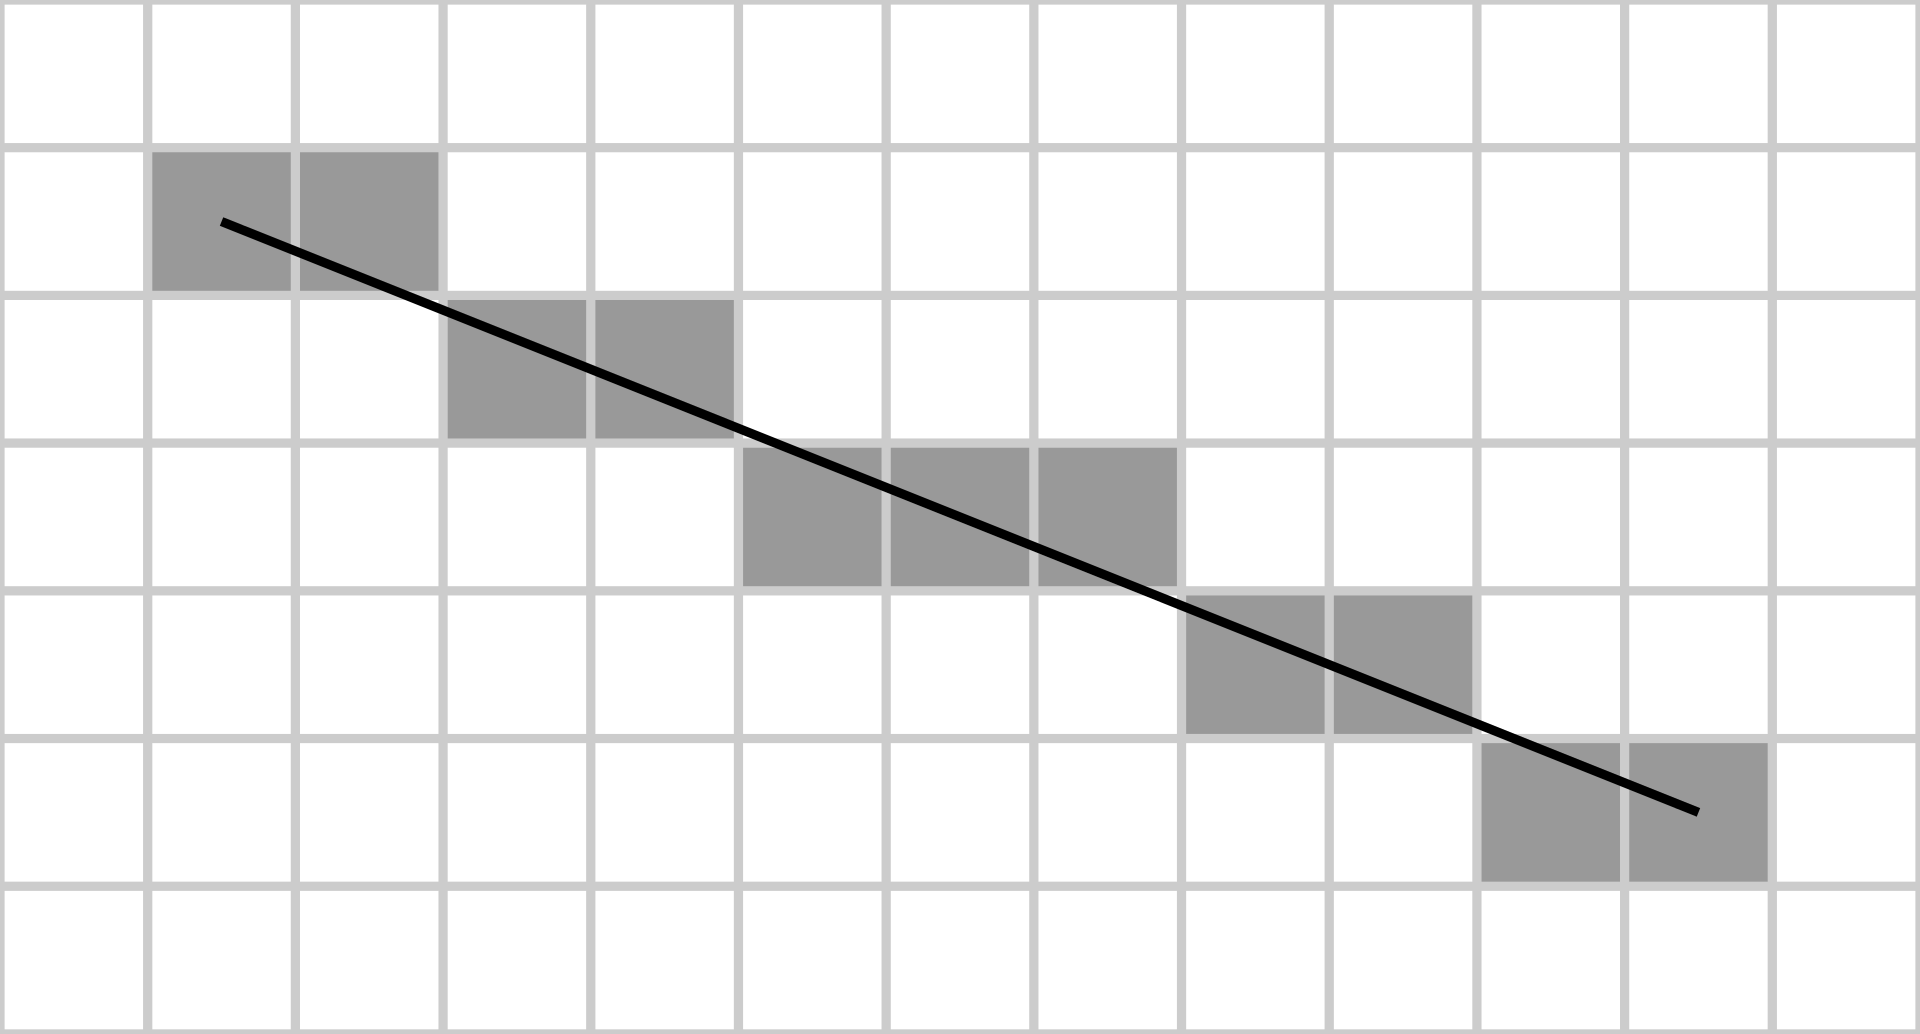
\includegraphics[width=8cm]{archivos/bresenham}
	\caption{Pintado de líneas en pantalla (adaptación de una línea a una cuadrícula) - Fuente: \href{https://en.wikipedia.org/wiki/Bresenham\%27s_line_algorithm\#/media/File:Bresenham.svg}{Wikipedia}}
	\label{fig:bresenham}
\end{figure}

En esencia, esta es la lógica que sigue el código de pintado:

\begin{itemize}
	\item Dados el punto de inicio y el punto de fin de la recta, calcular la pendiente de la recta a partir de los mismos.
	\item Si la pendiente es inferior a 45º, iterar desde el punto de inicio de la recta hasta el punto final, incrementando siempre la posición horizontal e incrementando sólo la posición vertical cuando el error acumulado es mayor que uno.
	\item Si la pendiente es superior a 45º, iterar desde el punto de inicio de la recta hasta el punto final, incrementando siempre la posición vertical e incrementando sólo la posición horizontal cuando el error acumulado es mayor que uno.
\end{itemize}

\begin{lstlisting}[style=C-color, caption={Versión simplificada y reducida del código para dibujar líneas en pantalla},label=cod:drawline]
void RenderLine(int x1, int y1, int x2, int y2, const Pixel &colour)
{
    float slope = GetSlope(x1, y1, x2, y2);

    //Slope < 45º
    if (slope <= 1.f)
    {
        DrawLineWithSmallSlope(x1, y1, x2, y2, colour, slope);
    }
    //Slope > 45º
    else
    {
        DrawLineWithBigSlope(x1, y1, x2, y2, colour, slope);
    }
}

void DrawLineWithSmallSlope(int x1, int y1, int x2, int y2, const Pixel &colour, float slope)
{
    float acummulatedError = 0.f;  
    int auxX = x1, auxY = y1; //auxiliar point that we will increment from the old point to the new one

    int signX, signY;
    GetSigns(x1, y1, x2, y2, signX, signY);

    //While we don't reach the desired pixel position
    while (auxX != x2 || auxY != y2)
    {

        RenderDot(auxX, auxY, colour);
        
        auxX += signX; //Increment X until it reaches the target

        acummulatedError += Fast::Abs(slope); //When this reaches 1, we increment Y

        if (acummulatedError >= 1.f)
        {
            auxY += signY;
            acummulatedError -= 1.f;
        }
    }
}
\end{lstlisting}

El código que se muestra en [\ref{cod:drawline}] es tan solo una versión simplificada, reducida y no funcional de la implementación en código del algoritmo para el dibujado de rectas en pantalla, pero que pretende ser suficiente para ejemplificar cómo se traduce la lógica anteriormente descrita al código.\\

Como se ha comentado previamente, este código se inspira en el algoritmo de Bresenham, pero no lo sigue. Una de las mayores diferencias es que el algoritmo de Bresenham sólo utilizaba números enteros, pues cuando fue desarrollado, las operaciones con números en coma flotante eran lentas y se realizaban por \emph{software}. Hoy en día, no obstante, se realizan por \emph{hardware}, y no suponen en muchos casos un coste significativo con respecto a las operaciones con enteros.\\

Además, según las necesidades han ido variando, se ha ido añadiendo funcionalidad adicional al pintado de líneas:

\begin{itemize}
	\item Posibilidad de definir un grosor de línea
	\item Posibilidad de definir un color de inicio y de final, sobre los que se interpola (dando una sensación de degradado)
\end{itemize}